%----------------------------------------------------------------------------------------
%	PACKAGES AND OTHER DOCUMENT CONFIGURATIONS
%----------------------------------------------------------------------------------------
%!TEX root = media_covid_knowledge.tex

\PassOptionsToPackage{unicode=true}{hyperref} % options for packages loaded elsewhere
\PassOptionsToPackage{hyphens}{url}
%
\documentclass[11pt]{article}
\usepackage{appendix}
\usepackage{lmodern}
\usepackage{amssymb,amsmath}
\usepackage{ifxetex,ifluatex}
%-------%
% Journal submission specifications - ASA format
%\usepackage{mathptmx}
%\usepackage[,bottom=1in,top=1in,left=1in,right=1in]{geometry}
\usepackage{geometry}
%\usepackage[doublespacing]{setspace} % alternate way to add double space
%\usepackage[document]{ragged2e} % do not right-justify text
%\usepackage{enotez}
%  \let\footnote=\endnote

%Running header
\usepackage{fancyhdr}
\pagestyle{fancy}
\fancyhf{}% Clear header/footer
\fancyhead[L]{Paying Attention to the Pandemic}
\cfoot{\thepage} %page numbers bottom center

% where figures/tables in document
%\usepackage[nolists,tablesfirst]{endfloat} % forces all floats to appear at end of document
\usepackage[section]{placeins} %keeps floats in place, using command \FloatBarrier
%\usepackage[nolists, tabhead, fighead]{endfloat}
%\usepackage{flafter} %force floats to appear after they are defined
%-------%

 % packages for figures
\usepackage{array}  % tables
\usepackage{wrapfig}  % wrap text around narrow tables or figures
\usepackage{graphicx}  % for inserting graphics from file
\usepackage{blindtext}
\usepackage{asymptote}
\usepackage{subcaption}
\usepackage{rotating} %landscape tables
\usepackage{geometry}
\usepackage{pdflscape}

% for figures in multiple parts
\usepackage{caption}
%\DeclareCaptionLabelFormat{cont}{#1~#2\alph{ContinuedFloat}}
%\captionsetup[ContinuedFloat]{labelformat=cont}

%Bibliography
\usepackage{natbib}
\setcitestyle{round,aysep={},yysep={,},notesep={:}}

\ifnum 0\ifxetex 1\fi\ifluatex 1\fi=0 % if pdftex
  \usepackage[T1]{fontenc}
  \usepackage[utf8]{inputenc}
  \usepackage{textcomp} % provides euro and other symbols
\else % if luatex or xelatex
  \usepackage{unicode-math}
  \defaultfontfeatures{Ligatures=TeX,Scale=MatchLowercase}
\fi
% use upquote if available, for straight quotes in verbatim environments
\IfFileExists{upquote.sty}{\usepackage{upquote}}{}
% use microtype if available
\IfFileExists{microtype.sty}{%
\usepackage[]{microtype}
\UseMicrotypeSet[protrusion]{basicmath} % disable protrusion for tt fonts
}{}
\IfFileExists{parskip.sty}{%
\usepackage{parskip}
}{% else
\setlength{\parindent}{0pt}
\setlength{\parskip}{6pt plus 2pt minus 1pt}
}
\usepackage{hyperref}
\hypersetup{
            pdftitle={Knowledge of COVID-19 and News Sources},
            pdfborder={0 0 0},
            breaklinks=true}
\urlstyle{same}  % don't use monospace font for urls
\usepackage{graphicx,grffile}
\makeatletter
\def\maxwidth{\ifdim\Gin@nat@width>\linewidth\linewidth\else\Gin@nat@width\fi}
\def\maxheight{\ifdim\Gin@nat@height>\textheight\textheight\else\Gin@nat@height\fi}
\makeatother
% Scale images if necessary, so that they will not overflow the page
% margins by default, and it is still possible to overwrite the defaults
% using explicit options in \includegraphics[width, height, ...]{}
\setkeys{Gin}{width=\maxwidth,height=\maxheight,keepaspectratio}
\setlength{\emergencystretch}{3em}  % prevent overfull lines
\providecommand{\tightlist}{%
  \setlength{\itemsep}{0pt}\setlength{\parskip}{0pt}}
\setcounter{secnumdepth}{0}
% Redefines (sub)paragraphs to behave more like sections
\ifx\paragraph\undefined\else
\let\oldparagraph\paragraph
\renewcommand{\paragraph}[1]{\oldparagraph{#1}\mbox{}}
\fi
\ifx\subparagraph\undefined\else
\let\oldsubparagraph\subparagraph
\renewcommand{\subparagraph}[1]{\oldsubparagraph{#1}\mbox{}}
\fi

% set default figure placement to htbp
\makeatletter
\def\fps@figure{htbp}
\makeatother

%----------------------------------------------------------------------------------------
%	DOCUMENT CONTENT
%----------------------------------------------------------------------------------------

\begin{document}

\title{Tentative Title: Paying Attention to the Pandemic: Knowledge of COVID-19 by News Sources and Demographics
\footnote{Corresponding Author: Molly M. King,
          Department of Sociology, Santa Clara University,
          500 El Camino Real, Santa Clara, CA, 95053.
          Email: mmking@scu.edu.}}

\author{Molly M. King \\ Department of Sociology, Santa Clara University}
\date{}

\clearpage\maketitle

%----------------------------------------------------------------------------------------
\section{Abstract}\label{sec:abstract}
%----------------------------------------------------------------------------------------
\pagestyle{fancy} %Running header
\setcounter{page}{1} %resets page number to 1

Never before has so much information been so immediately accessible to
so many. Yet the challenges in sorting through this information are perhaps
greater than ever. Previous research has looked at the role of social media and
other news sources on shaping the U.S. population’s understanding of the COVID-19
pandemic. However, what has not been studied is how this knowledge acquisition
is structured by the demographic characteristics of gender, race and ethnicity, and
income. Furthermore, how does uncertainty about this knowledge also differ by
demographic group membership? This study reveals how the use of
different news sources differentially shape access to accurate information about
COVID-19 and related topics for different demographics. I answer these questions
by analyzing recent Pew Research survey data asking respondents about their news
media consumption and their knowledge of COVID-19 science and related current
events information. I determine the effect of demographic group memberships in
shaping (mis)information and (un)certainty about COVID-19 received through news sources.


\section{Keywords}

knowledge, inequality, media, COVID-19

\newpage

%----------------------------------------------------------------------------------------
\section{Introduction}\label{sec:introduction}
%----------------------------------------------------------------------------------------


Never before has such a wealth of information been so immediately accessible to
so many. Yet the challenges in sorting through this information are perhaps
greater than ever \citep{Metaxa-Kakavouli2017}.
Correct and incorrect factual knowledge shaped the
2016 U.S. election cycle \citep{Allcott2017, Gunther2017} and promise to shape
politics for years to come. Topics many believe to be objective and resolved
after years of scientific consensus are now resurfacing as topics of factual
debate \citep[e.g.,][]{Hmielowski2014}. Command over information matters for a
great many outcomes \citep{Webster2006}. Social media platforms play an increasingly important role in
what we perceive as true. This paper investigates how demographic categories
influence accurate understanding of the facts about COVID-19, and how this
varies by news source.

I determine the effect of demographic group memberships in shaping
(mis)information about COVID-19 received through news sources. This research
project has important implications for sociology, technology, and information
studies. Understanding how misinformation breaks down along class, gender, and
race and ethnicity lines makes it a contribution in the style of Mannheim's
sociology of knowledge \citep{Mannheim1929,Swidler1994}.


%-------------------------
\subsection{Information Inequalities}

In the context of COVID-19 knowledge, there are two reasons why we might
be concerned about differential access to correct facts:

\begin{enumerate}
\def\labelenumi{(\arabic{enumi})}
\item
  Differences in the amount of information people have are influenced by
  unequal social positions in our society; and
\item
  Information is a potential cause of later inequality in outcomes and
  access to resources.
\end{enumerate}

Many studies have evaluated information seeking behaviors and needs
\citep{Case2016}. Researchers have sought to understand what contributes to the information divide
and the resulting states of advantage and disadvantage. For a person to be
informationally advantaged, they need not only the economic capital for
information access, but also the intellectual resources for information
gathering, processing, and assessment \citep{Sweetland1993}. In this way,
information filtering skills are key. Information overload, in certain contexts,
can thus actually create information poverty rather than making people
information rich \citep{Yu2006}. In the modern context, skill spillovers from
knowledge work may give some groups more abilities than others. Those who use
information sorting skills in their occupations may be more able to use these
abilities to benefit their private lives, as well \citep{Xanthopoulou2012}.

The information divide can be defined as ``inequality in the possession and usage of
information and communication sources in a particular society''
\citep{VanDijk1997,VanDijk2000}. Various terms have been used by researchers to characterize this information
divide and the resulting state of deprivation for those in less advantaged
positions. One of the more sociological definitions is offered by Britz and
colleagues, who argue that information poverty is based on an interrelated
set of knowledge, information, and information infrastructures:

\noindent\begin{minipage}{\linewidth}
\begin{quote}
  [A] situation in which individuals and communities, within a given context, do
  not have the requisite skills, abilities or material means to obtain efficient
  access to information, interpret it and apply it appropriately; [information
  poverty] is further characterized by a lack of essential information in a
  poorly developed information infrastructure. \citep[194]{Britz2004}
\end{quote}
\end{minipage} \\

Information inequalities are the product of the unequal distributions of information resources.
Where might systematic variations in the distribution of
information by demographic characteristics come from? Understanding the causes
at the root of information differences can point to systemic inequities in societal institutions, such as the media.

%-------------------------
\subsection{Inequalities \& Media Consumption}

The vertical (or hierarchical) perspective on information equity associates
better information access and use with greater socioeconomic advantages
(individual or group demographics). The most socioeconomically advantaged
members of society are therefore more likely to have better information access
and use. Information is viewed as a private good or commodity. The vertical
theory holds that knowledge is a resource that can be traded and distributed,
and there is a mutually agreed-upon value hierarchy among information
categories. This form of knowledge inequality could be ameliorated through the
more equitable allocation of socioeconomic resources.

The horizontal perspective, in contrast, views knowledge categories as
subjectively and socially constructed. Information is a public good. Under this
view, the value of information is subjective and context-dependent
\citep{Lievrouw}. As such, information advantages are the result of groups'
differential behaviors, which create the context for which information is most
important for that group. People may have different ``interests, concerns,
expertise, experiences, and social contexts that affect their requirements for
and uses of information, even within the same community, economic, or ethnic
group'' \citep[501]{Lievrouw}. The inequality is horizontal because there is
little agreement over which types of knowledge are most important. Under the
horizontal approach, the ``fairness or equity of access and use, rather than the
more or less equal distribution of information goods, may be a more useful
foundation for studying inequities'' and rectifying them \citep[501]{Lievrouw}.




%[Example studies on info inequality here from diss papers]

What these studies tell us is that demographic gaps (gender and race/ethnicity)
in knowledge cannot be explained entirely by the usual suspects. Even after
controlling for income and educational attainment, large gaps remain.
Understanding the influence of demographic status characteristics on information
inequality not only helps us understand the state of misinformation in the U.S.,
it also lays the groundwork for the future study of potential causes.

Research on algorithmic bias in ad delivery reveals widespread implicit and
explicit discrimination \citep{Sweeney2013}. The distribution of attention on
the World Wide Web also concentrates attention on fewer sites each year,
reducing entropy and increasing the Gini coefficient, creating an effective size
of fewer than 20,000 websites \citep{McCurley2007}. However, we do not know how
this demand for attention is spread across the population, nor do we know how it
may differentially affect the information people of different demographic status
groups receive over time.


We do know that different demographics are more likely to consume different types of news. For example, older adults follow more local news and more highly educated adults are more likely to follow international news \citep{Mitchell2018}. Local news is viewed as more trustworthy than national news, particularly among Democrats \citep{KnightGallup2019}.

-does national news cater to a majority white audience?


%-------------------------
\subsection{Media Consumption \& Misinformation}

%INFO - NEWS SOURCE - DEMOGRAPHIC (pre-pandemic)
We know a bit about these dynamics before the COVID-19 pandemic.

-political sociology of local news:
--from fake local news conglomerates
--decentralized versus centralized new sources
--what is meaning of friends and family? not getting any news at all?

%Search Engines
Search engines play an increasingly important role in what we perceive as true (CITE). To my knowledge, no research has been done to look at how this impacts people over time or differs by demographic characteristics.

An increasing number of Americans get their news from YouTube
\cite{Shearer2017}, making this an ever more important system to understand with
respect to misinformation.

%Social Networks
Information also spreads through social networks online. People ``are probabilistically influenced to adopt the opinions of their neighbors, and can promote their own opinions by being reluctant to change them. In this way, an intransigent minority can convert the entire group over to their minority opinion'' \citep{West2011}. In this way, strongly opinionated minority group members can have a strong influence in what is essentially a very small information ecosystem in the World Wide Web. For example, influential figures in the alternative conservative media network promote a stepwise radicalization process amongst more moderate conservatives: ``when libertarian and conservative influencers invite white nationalists onto their channels, they expose their audiences to alternative frameworks for understanding the world. Thus, audiences may quickly move from following influencers who criticize feminism to those promoting white nationalism. This is why the high concentration of the networking between influencers can prove so powerful'' \citep{Lewis}.

In short, psychological and cognitive biases \citep{DiMaggio1997} are colliding with the technological realities of our time to create novel knowledge inequities \citep{Mohammed2012}.


%-------------------------
\subsection{Demographics, Information Behavior, \& Misinformation}


%-------------------------
\subsection{COVID-19 \& Misinformation}

We know from research in several domains that gaps in information produce
inequalities in later outcomes. Aside from their role in producing status
differences that have consequences in everyday lives
\citep{Ridgeway2014,KingGender}, differences in knowledge may also result in
concrete access to other resources. In the case of correct knowledge about
COVID-19, we might imagine that those with the most correct knowledge might be
more likely to have positive health outcomes during the pandemic (CITE). Many
would find this even more normatively problematic if those types of information
which historically marginalized groups have the least access to correspond to
the types of information which tend to provide access to important other
resources (such as health, economic or material goods).

%COVID / TECH ACCESS & INEQUALITY
More recently, researchers are looking at the implications of this differential
access to accurate information on consequences for schooling, employment, and health
during the COVID-19 pandemic.

%Health outcomes




%-------------------------
RESEARCH QUESTION
But to my knowledge, no one has yet investigated the consequences of different
demographics on differential information availability on the internet and on
misinformation spread through social media and other new sources during the COVID-19 pandemic.
How is knowledge structured by the demographic characteristics of gender,
race/ethnicity, and income? How does uncertainty about this knowledge also
differ by demographic group? And how does use of different news sources
differentially shape access for different demographics?


%----------------------------------------------------------------------------------------
\section{Methods}\label{sec:methods}
%----------------------------------------------------------------------------------------

\subsection{Data}\label{sec:data}

In this analysis, I investigate factual (mis)information and uncertainty using
the Pew Pathways June 2020 American Trends Panel Wave 68 Survey (CITE). The
survey features four questions of particular interest, which ask about factual
knowledge about the COVID-19 pandemic and the economy during this time:

\begin{enumerate}
\def\labelenumi{(\arabic{enumi})}
  \item ``As far as you know, are antibody tests for the coronavirus (also known as serology tests) intended to detect…'' (Correct answer is ``A previous infection'')
  \item ``Do you happen to know who Anthony Fauci is?'' (Correct answer is ``An infectious disease expert and government health adviser.q)'
  \item ``As far as you know, how did states in the U.S. respond during the coronavirus outbreak?''" (Correct answer is ``Some states in the U.S. have not had a statewide stay-at-home order.'')
  \item ``Is the national unemployment rate as reported by the government currently…'' (Correct answer is 15\%)
\end{enumerate}

My analysis also includes basic demographic variables for respondents, including
gender, race and ethnicity, income, age, and educational attainment. So that
readers can see all analysis decisions for themselves, all annotated code is
available at my Open Science Framework project page:
(URL removed for blinded review).
%\url{https://osf.io/qf624/}.


%-------%
\subsubsection{Gender}\label{sec:gender}

Gender and sex are not binary designations, but rather lie along a flexible
spectrum or at least exist in multiple categories \citep{Connell2002b,
Fausto-Sterling1993, Fausto-Sterling2000, West1987, Maglioizzi2016}.
However, the available data have only categories of `woman' or
`man.' Therefore, I code gender as a binary variable.

%-------%
\subsubsection{Race and Ethnicity}\label{sec:race-and-ethnicity}

Measurement of race is another area in which best practice\footnote
  {Beginning in 2000, the U.S. Census moved from allowing people to choose only
  one racial category identity to allowing people to choose as many racial
  categories as they identified with \citep{OfficeofManagementandBudget1997,
  OfficeofManagementandBudget2000}.}
is often limited by available data. I code the racial categories of non-Hispanic
White, non-Hispanic Black/African-American, and non-Hispanic Asian, the ethnic
category of Hispanics who do not identify with any of the other racial
categories, and the category of `other.' This race `pentagon' classification has
been found most useful in explaining variation in education and income (compared
to either a seven or eight category, tri-racial, or skin tone classification
system) \citep{Howell2017}.

%-------%
\subsubsection{Socioeconomic Class: Income}\label{sec:class-income}

Social class both creates and is produced by differences in knowledge. I use
income as my primary measure of social class. This is an imperfect measure, to
be sure, and others (such as parental occupation data) would be preferable for
both their causal separability\,---\,given the temporal antecedence of parental
occupation,\--\,and their empirical validity \citep{Weeden2005a, Weeden2012}.
However, parental occupation is not available for these data. An analysis of the
association of income and knowledge is thus best understood as an analysis of
which knowledge is crucial to socioeconomic elites.

I choose family income rather than individual (personal) income because it
more accurately reflects the total resources available to the individual, and
therefore are a better reflection of socioeconomic status.\footnote
  {The reliability of self-reported income typically ranges from 71\% to 98\%,
  with a mean of 86\% \citep{Marquis1986}. In other words, if the same
  individuals are asked about their income at two different points in the survey
  using two slightly different measures to get at the same question, the results
  will agree, on average, within about 0.86. Compared to tax or Social Security
  Administration records, self-reported measures of income tend to be about 70
  to 78\% of official amounts \citep{Coder1996, Reardon2011a}.}
I transform categorical income into continuous income in order to make
regression coefficients more interpretable. A continuous measure of income is
more intuitive to interpret than categorical income bins. Therefore, I use the
Random Empirical Distribution Imputation (REDI) method to convert the Pew
categorical family income data into continuous income estimations
\citep{KingREDI}. For each category of family income, I randomly draw the same
number of observations from within those same bounds in the Current Population
Survey March Annual Social and Economic (CPS ASEC) supplement \citep{ASEC2018}.
I then apply these exact family income values from the CPS ASEC to the
corresponding set of categorical values within the original Pew survey. Thus, I
get a distribution of numerical values in the original Pew survey that
corresponds to their probability of occurrence in the CPS ASEC. Repeating this
for all income categories provides continuous cold-deck imputed income values
for every respondent. I used this method rather than assigning the midpoint
value to preserve variance and keep information from the extreme income
categories. For more details on the conversion of categorical to continuous
family incomes, see \citet{KingREDI}.

%https://stats.stackexchange.com/questions/143110/when-to-use-log-in-regression
To aid interpretation, I take the natural log of the family income. Thus, the
control variable may be interpreted as the impact of a one percent increase in
family income on the odds (or log odds) of knowing the correct answer.

%-------%
\subsubsection{Age}\label{sec:age}

I restrict my analyses to adults ages 18 and over.  Pew provides only
categorical age, in predefined groups: 18-29; 30-49; 50-64; and 65 and over.

% Since Pew provides only categorical age, I also use the REDI method
% \citep{KingREDI} to convert age to a continuous variable. I calculate the number
% of respondents in each age category, and pull at random an equivalent number of
% observations within that age range from the CPS ASEC. I take the exact age value
% of that observation from the CPS ASEC and assign the age value as if it were the
% original respondent's exact age. Again, this preserves variance in the age
% distribution.

There are of course different kinds of things people are expected to know at
different life stages. However, there is no reason to expect that the rate of
accumulation of knowledge should vary based on any of my other covariates.
Therefore, I include age as a regressor in my models, but I do not include any
interaction variables.
%But the kinds of things women and men expect to learn at different  of lifestages are likely to be different ...

%-------%
\subsubsection{Education}\label{sec:ducation}

Education categories are collapsed to four categories (less than high school,
completed high school, some college, and bachelor's degree or more). Though some
studies provide more fine-grained detail\,---\,including either the precise number
of years of education or additional possible educational degrees like
Associate's or technical school\,---\,these four categories are present in all
surveys.



\subsubsection{News}
After initially analyzing the models with all news source categories separate
(results available in online appendix), I grouped news sources together based on
their structurally similar roles. This grouping was meant to facilitate the
application of interaction terms and interpretation of results. The substantive
interpretation of model results prior to the addition of interaction terms to
the model remain unchanged between the separation of each unique news source and
the combination of socially similar sources.

The sources were combined in the following way: International and national news
were combined into a single variable; local news remained separate for analysis;
all political sources of COVID-19 information were combined, including Trump and
his coronavirus task force, Joe Biden and his campaign, and State and local
elected officials and their offices; and public health organizations and
officials remained a separate variable. Finally, I created a single variable
representing informal networks, including the original variables representing
information received from friends, family and neighbors; community or
neighborhood newsletters or listservs; and online forums or discussion groups.


 %-------%
\subsection{Model}\label{sec:model}

I use a two-step model to analyze the levels of uncertain and correct answers
for the three factual knowledge question in this study
(Figure~\ref{fig:TwoStepModelOfKnowledge}).


\begin{figure}[ht]
  \begin{center}
    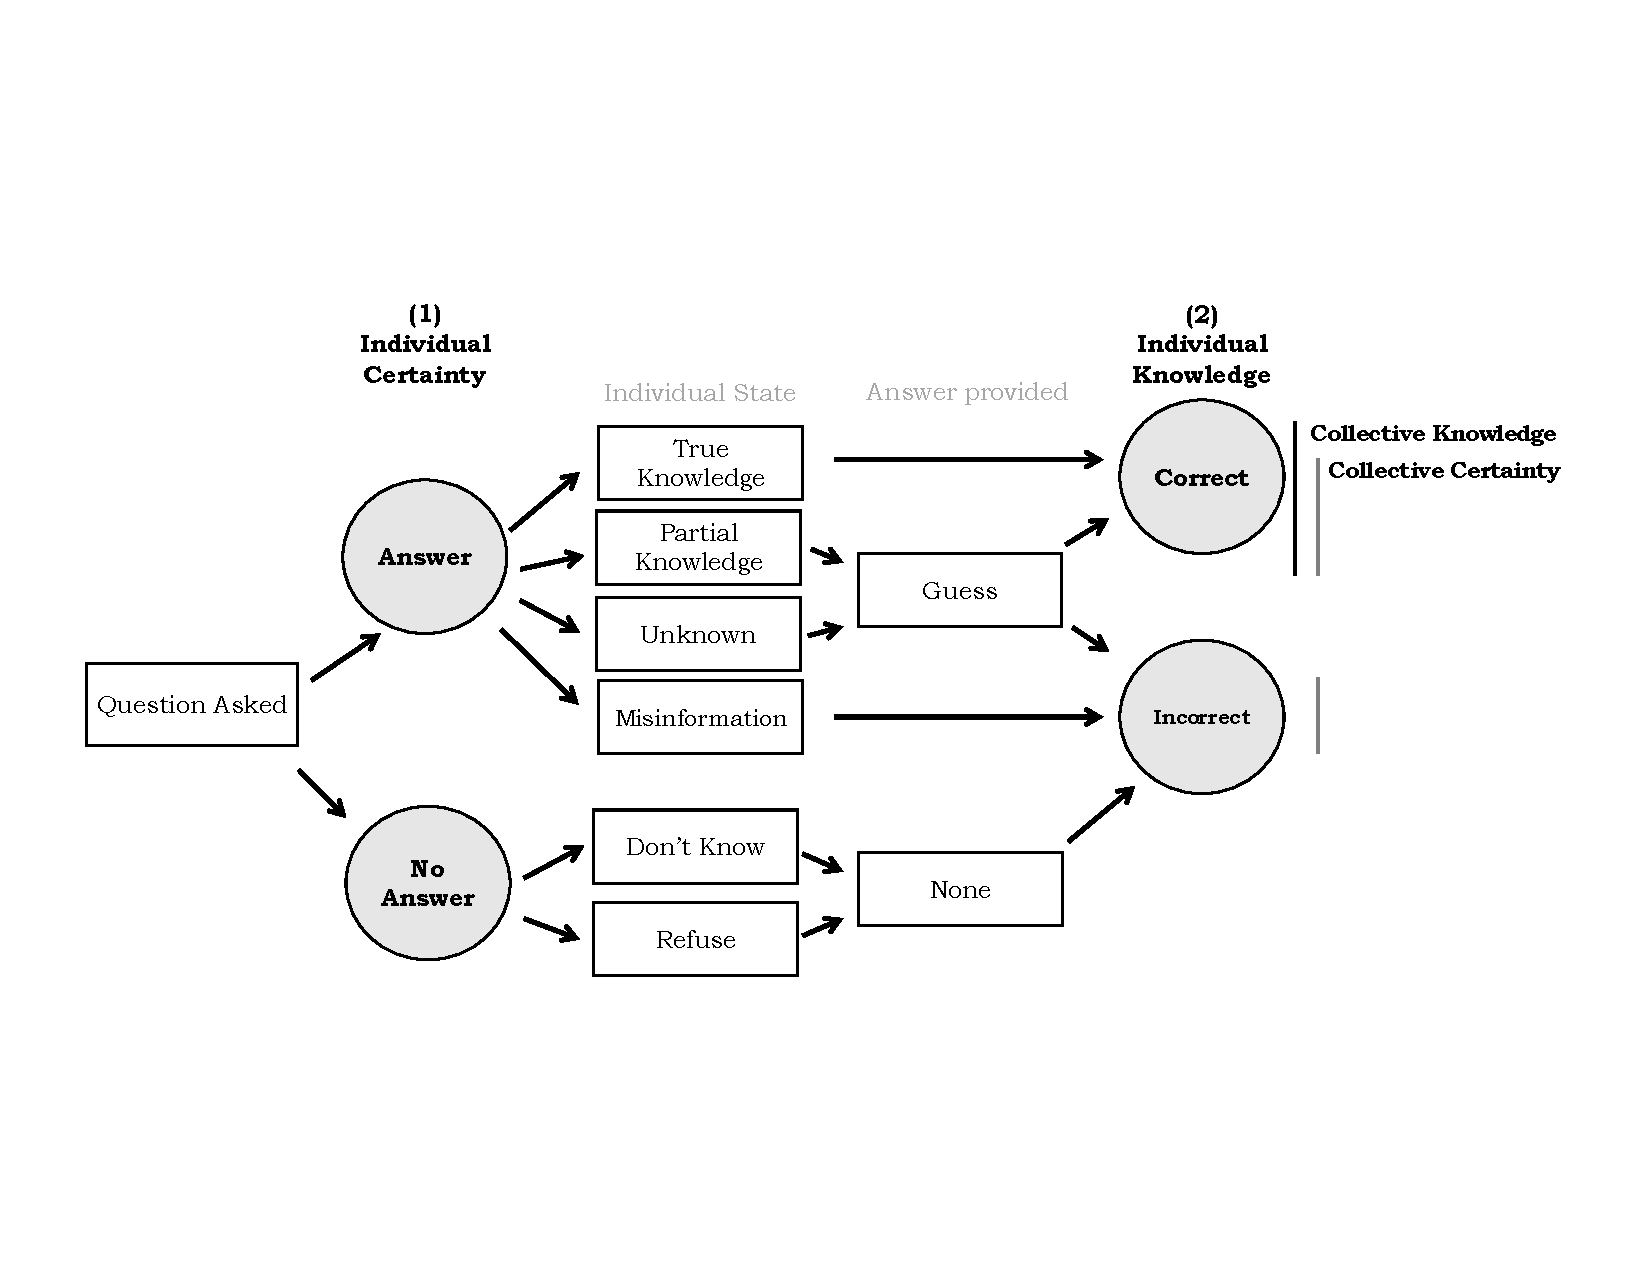
\includegraphics[width=1.0\textwidth]{/Users/mollymking/Documents/Documents/SocResearch/COVID_Knowledge_News/covid_knowledge_news/figures/two-step-model-of-knowledge}
  \end{center}
  \caption[A model of responses to knowledge questions]
  {\emph{A model of responses to knowledge questions.}
   My analytical approach conceives of respondents following a two-step decision
   process when answering factual knowledge questions in surveys. First, the
   respondent decides if they are sufficiently certain to answer the question or
   not (a measure of collective certainty when aggregated). Others answer the
   question either `don't know' or some variation thereof. Conditional on
   answering, the respondent proceeds to step two, either getting the question
   correct or incorrect (a measure of misinformation).}
  \label{fig:TwoStepModelOfKnowledge}
\end{figure}


I separate my model of knowledge into two steps (see
Figure~\ref{fig:TwoStepModelOfKnowledge}). First, I analyze the proportion of
respondents who are uncertain about each factual knowledge question by domain.
To do this, I estimate the weighted population mean for the response of `don't
know' (or similar answers such as `not sure,' `no opinion,' `prefer not to say,'
and `don't know / refused') for each knowledge question where such an answer was
available to the respondent:

 $$ mean_{DK} = \frac{P(y = 1)}{N}. $$

In this model, \emph{y = 1} is the outcome variable (`don't know' answer), and
\emph{N} is the size of the dataset. The mean value `don't know' for the population for a single knowledge
question ($mean_DK$) is equal to the survey-weighted probability of the
respondent answering `don't know' (or a variant) divided by the total number of
survey respondents who were asked the question. Respondents who refused to answer are excluded from the analysis.

Second, I analyze the proportion of the population (out of those providing an answer related to the substance of the
question) who answered correctly and incorrectly. To do this, I estimate the
population mean (and standard error) for the binary variable indicating correct
answer:

 $$ mean_C = \frac{P(y = 1)}{N}. $$

In this model, \emph{N} is the size of the dataset, and \emph{y = 1} the outcome
variable (correct answer). The probability of answering correctly ($P(y = 1)$)
is calculated out of all individuals who provided a correct or incorrect answer and those who respond
`don't know'. Respondents who refused to answer are excluded from the analysis.
Hence, the mean value correct for the population for a single knowledge
question ($mean_C$) is equal to the survey-weighted probability of the
respondent getting the knowledge question correct divided by the total number of
survey respondents.



%-------%
\subsection{Descriptive Findings}\label{sec:descriptives}

Summary statistics for each of these factors related to the three knowledge questions are presented in Table%~\ref{table:SummaryStats}.

% Table) Summary Statistics

% %this is all to turn table horizontal and clean page
% \newpage
% \newgeometry{margin=1in} % modify this if you need even more space
% \begin{landscape}
% \thispagestyle{empty}
%
%
% \begin{table}
%   \caption[Descriptive statistics for predictors of correct COVID-19 knowledge.]
%   {\emph{Descriptive statistics for predictors of correct COVID-19 knowledge: mean (standard deviation). }}
%   \label{table:SummaryStats}
% %  \small
%   \begin{tabular}{l|c|c|c|c}
%     \hline   % adds horizontal lines to the top of the table
%                           & Anthony Fauci            & Antibody tests          & Unemployment      & Some states\\
%                           & is an infectious disease & detect previous         & rate around 15\%  & had no stay-at- \\
%     Variable              & expert \& govt. adviser  & coronavirus infections  & in June           & home order \\
%     \hline
%     \multicolumn{4}{l}{{\bf News Source} }   \\
%       \enspace International news outlets &               &                    &                   &                \\
%       \enspace National news outlets &                    &       &   &    \\
%       \enspace Local news outlets    &                    &       &   &    \\
%       \enspace Trump or coronavirus  &                    &       &   &    \\
%       \enspace task force            &                    &                    &                   &      \\
%       \enspace Biden campaign        &                    &       &   &    \\
%       \enspace State and local       &                    &       &   &    \\
%       \enspace elected officials     &                    &                    &                   &       \\
%       \enspace Public health         &                    &       &   &    \\
%       \enspace orgs. \& officials    &                    &                    &                   &       \\
%       \enspace Friends, family       &                    &       &   &    \\
%       \enspace \& neighbors          &                    &                    &                   &       \\
%       \enspace Community or          &                    &       &   &    \\
%       \enspace neighborhood news     &                    &                    &                   &       \\
%       \enspace Online forums         &                    &       &   &    \\
%       \enspace or discussion groups  &                    &                    &                   &      \\
%     \multicolumn{5}{l}{{\bf Race} }   \\
%       \enspace White                 &                    &       &   &    \\
%       \enspace Black                 &                    &       &   &    \\
%       \enspace Asian                 &                    &       &   &    \\
%       \enspace Hispanic              &                    &       &   &    \\
%       \enspace Other/Mixed           &                    &       &   &    \\
%     \multicolumn{5}{l}{{\bf Income}}   \\
%       \enspace \$0 to \$10,000       &                    &       &   &    \\
%       \enspace \$10,000 to \$20,000  &                    &       &   &    \\
%       \enspace \$20,000 to \$30,000  &                    &       &   &    \\
%       \enspace \$30,000 to \$40,000  &                    &       &   &    \\
%       \enspace \$40,000 to \$50,000  &                    &       &   &    \\
%       \enspace \$50,000 to \$75,000  &                    &       &   &    \\
%       \enspace \$75,000 to \$100,000 &                    &       &   &    \\
%       \enspace \$100,000 to \$150,000 &                    &       &   &    \\
%       \enspace \$150,000 and above  &                    &       &   &    \\
%     \hline  % adds horizontal line to the bottom edges
%     N                     & 9173                     &  9173                   &   9173            &  9173 \\
%     \hline
%   \end{tabular}
% \end{table}
%
% \end{landscape}
% \restoregeometry
\newpage





%-------%
\subsection{News Source}\label{sec:news source}





%-------%
\subsection{Race, Ethnicity, and News Source}\label{sec:race-news}

%interactions of race and news source


%-------%
\subsection{Income and News Source}\label{sec:income-news}

 income and news source



%----------------------------------------------------------------------------------------
\section{Discussion \& Conclusions}\label{sec:conclusion}
%----------------------------------------------------------------------------------------

This paper describes the current state of COVID-19 knowledge in the U.S. as a
function of demographic characteristics and news consumption. This makes it a
contribution in the style of Mannheim's sociology of knowledge
\citep{Mannheim1929,Swidler1994} and the study of demographic inequalities in
gender, class, and race/ethnicity. These are all important implications of
knowledge inequality and important reasons compelling its relevance to scholars
of inequality and policy-makers.

Individuals face the world with different sets of knowledge, shaped by their
social contexts. Some of this knowledge may be correct, and some of it may be
incorrect, as we see in the results of this analysis. People may be aware that
some of their incorrect knowledge represents a gap in their understanding, but
in other domains, they may falsely believe what they know is the truth.


Misinformation is an important emerging topic in
information science and sociology \citep{Metaxa-Kakavouli2017}. In essence, this
is a study of modern epistemology. How do we come to know what we know? How do
we come to be misinformed? Both, often through engagement with internet news
sources and social media. If our news media and other sources of factual
information are pushing users in biased ways and ways that depend on the
demographics of the user, then we cannot be assured that this information is
reliable. Understanding how this differs by demographic variables has important
implications for social research and policy.

Democracy depends on collective decision-making, which in turn depends on trust
in institutions and access to reliable information, regardless of political
persuasion. If our search engines and recommendation algorithms are pushing
users in biased ways and ways that depend on the demographics of the user, then
we cannot be assured that this information is reliable. Once we better
understand the ways our media are shaping information consumption and knowledge,
we can design better systems to reduce bias in these sociotechnical
institutions. This research project will provide concrete evidence on different
groups' command over information resources, a matter of increasing importance in
modern society. It aims to understand how identity categories influence
consumption of information online.




%----------------------------------------------------------------------------------------
\section{Data Availability}\label{sec:data-availability}
%----------------------------------------------------------------------------------------

The project described in this paper relies on publicly available data from
surveys administered by the Pew Research Center.
In keeping with recommendations on transparent and open social science
\citep{Freese2018}, all code used to analyze these data are available at the
Open Science Framework project repository at [redacted for blind review].
%\url{DOI.ORG/10.17605/OSF.IO/QF624}.


%----------------------------------------------------------------------------------------
\section{Acknowledgments}\label{sec:acknowledgments}
%----------------------------------------------------------------------------------------

The author gratefully acknowledges Christof Brandtner for helpful comments on
earlier drafts of this paper.


%----------------------------------------------------------------------------------------
\subsection{Funding}\label{sec:funding}
%-------------------------------------------
This work was supported by funding from Santa Clara University.


%------------------------------------------------------------------------------
\newpage
\hypertarget{references}{%
\label{references}}
\renewcommand{\bibname}{References}

\bibliographystyle{/Users/mollymking/Documents/SocResearch/LatexStyleFiles/asa} %tells to use asr style file instead of natbib
\bibliography{/Users/mollymking/Documents/SocResearch/Mendeley/library}

%----------------------------------------------------------------------------------------

\end{document}
